\documentclass[10pt, a4paper, twocolumn]{article}
\usepackage[utf8]{inputenc}
\usepackage{graphicx}
\usepackage{geometry}
\usepackage{times}
\usepackage{cite}
\usepackage{amsmath}
\usepackage{amssymb}
\usepackage{booktabs}
\usepackage{multirow}
\usepackage{url}
\usepackage{hyperref}
\usepackage{enumitem}
\usepackage{tikz}
\usetikzlibrary{positioning, fit, backgrounds}
\usepackage{xcolor}
\usepackage{algorithm}
\usepackage{algpseudocode}
\usepackage{caption}
\usepackage{subcaption}

\DeclareUnicodeCharacter{0001}{}

\geometry{top=2cm, bottom=2cm, left=1.5cm, right=1.5cm}
\setlength{\emergencystretch}{3em}
\sloppy
\hfuzz=30pt
\hbadness=10000

\hypersetup{
    colorlinks=true,
    linkcolor=blue,
    citecolor=blue,
    urlcolor=blue
}

\title{\textbf{MANJU: A Multi-Agent Framework for Natural Just-in-Time Understanding in Thai Voice-Based Customer Service}}

\author{
    Sawit Koseeyaumporn, Siratee Saiprom, Sansiri Tarnpradab \\
    \textit{Department of Computer Engineering} \\
    \textit{King Mongkut's University of Technology Thonburi} \\
    \textit{Bangkok, Thailand} \\
    \texttt{\{sawit.kosee, siratee.saip, sansiri.tar\}@kmutt.ac.th}
}

\date{}

\begin{document}

\maketitle

\begin{abstract}
This paper presents \textbf{MANJU} (Multi-Agent AI for Natural
Just-in-Time Understanding), an automated platform for Thai-language
customer service delivered through real-time voice interaction.
MANJU transcribes a customer's spoken query, applies multi-agent
reasoning with retrieval-augmented generation (RAG) to determine the
optimal response strategy, and synthesises a reply in natural
Thai---all within five seconds.
A visual drag-and-drop workflow editor enables non-technical operators
to compose and modify conversation logic without programming.

Evaluated on 50 Thai customer-service queries, MANJU achieves 94\%
intent routing accuracy and improves factual groundedness from 50\%
to 88\% with RAG enabled, with end-to-end latency consistently within
the five-second design target and faster-than-real-time speech
synthesis (RTF\,=\,0.42).
\end{abstract}

\vspace{0.5em}
\noindent\textbf{Keywords:} Multi-Agent System, Voice AI, Thai NLP,
Retrieval-Augmented Generation, Customer Service Automation.

% ===========================================================================
\section{Introduction}
% ===========================================================================

Enterprises increasingly face pressure to provide uninterrupted customer
support, yet telephone-based service consistently underperforms during
peak demand due to insufficient staffing, extended queue times, and
consequent customer attrition~\cite{gans2003callcenters}.
Existing AI deployments partially address this gap, but remain limited to
text-only chatbots or rule-based interactive voice response (IVR) systems
that follow rigid decision trees.
Neither paradigm supports natural voice dialogue in Thai, dynamic knowledge
retrieval, or flexible adaptation to diverse business
domains~\cite{manjuProgReport}.

This paper introduces \textbf{MANJU}, a voice-based customer service
platform designed specifically for the Thai language.
Upon receiving a spoken query, MANJU transcribes the input, applies
multi-agent reasoning to determine the optimal response strategy, retrieves
supporting evidence from domain-specific documents when required, and
synthesises a reply in natural Thai---all within five seconds.
A distinguishing feature of MANJU is that the complete conversation logic
is configured through a visual workflow editor requiring no programming
knowledge, enabling rapid deployment by non-technical operators.

Our principal contributions are:
(i)~a \textbf{visual, no-code workflow builder} delivered as a web application, enabling non-technical operators to design and deploy conversation flows via drag-and-drop without programming;
(ii)~a \textbf{multi-agent orchestration engine} in which specialised agents for intent classification, document retrieval, live data lookup, and response generation cooperate within a RAG-grounded pipeline; and
(iii)~a \textbf{production-ready Thai voice platform} with streaming ASR, GPU-accelerated TTS with voice cloning, and a secure four-tier containerised deployment.

\noindent\textbf{Paper Organization.}
Section~\ref{sec:related} reviews related work.
Section~\ref{sec:methodology} describes the MANJU framework.
Section~\ref{sec:experiments} presents results.
Section~\ref{sec:conclusion} concludes.

% ===========================================================================
\section{Related Work}
\label{sec:related}
% ===========================================================================

\subsection{Automatic Speech Recognition}
ASR converts speech signals into text using deep learning.
A typical pipeline digitizes audio, extracts acoustic features (e.g., mel-spectrograms), and decodes text via an encoder-decoder or transducer model.
Large-scale end-to-end models such as OpenAI Whisper~\cite{radford2022whisper} demonstrate broad multilingual robustness; however, their non-causal encoder-decoder architecture introduces fundamental limitations for streaming applications: reliance on future context, chunking artifacts that split words, overlapping re-processing overhead, and unpredictable latency from autoregressive decoding.

Of particular relevance to MANJU is Typhoon ASR Real-Time~\cite{sirichotedumrong2026typhoonasr}, a 115M-parameter FastConformer-Transducer model for low-latency Thai streaming ASR.
Unlike offline Whisper-based approaches~\cite{tipaksorn2024pathumma,aung2024thonburian}, its Transducer (RNN-T) decoder enables frame-synchronous streaming without chunking latency.
Trained on approximately 11{,}000 hours of Thai audio, it achieves 6.81\% CER at 4{,}097$\times$ real-time throughput (15--19$\times$ faster than Whisper) at \$0.0023/hr on an L4 GPU, making it the target server-side upgrade for MANJU (Section~\ref{sec:conclusion}).

\subsection{Text-to-Speech Synthesis}
Because MANJU delivers its responses as spoken Thai audio, the quality and speed of the synthesis stage directly affect user experience.
Modern end-to-end TTS systems predict acoustic features and synthesise waveforms via neural vocoders~\cite{tan2021ttssurvey}.
Qwen3-TTS-12Hz-1.7B supports three voice modes---base voice cloning, configurable preset voices, and text-described voice design---enabling diverse speaker personalisation within a 1.7B-parameter architecture accelerated by Flash Attention~2~\cite{dao2022flashattention}.
MANJU adopts Qwen3-TTS as its primary synthesis backend to enable on-premise Thai voice cloning without cloud dependency.

\subsection{Multi-Agent Orchestration and Retrieval-Augmented Generation}
Transformer-based LLMs~\cite{vaswani2017attention} model long-range token dependencies for contextual language understanding and generation.
In customer service, LLMs interpret user intent, generate coherent responses, and integrate external knowledge through in-context grounding.
Qwen3.5~\cite{qwen2025qwen35} is an open-weight instruction-following model that supports multilingual tasks---including Thai---and enables on-premise deployment without API dependency, reducing operational cost and data-privacy exposure.
MANJU adopts Qwen3.5 as its default reasoning backbone, with configurable LLM selection per workflow node via LiteLLM provider abstraction.

However, a single monolithic LLM cannot reliably separate heterogeneous subtasks such as intent classification, document retrieval, live data lookup, and response generation, which exhibit distinct failure modes and benefit from explicit delegation to domain-specialised components~\cite{langgraph2024}.
Multi-agent architectures address this by decomposing complex reasoning into specialised agents that coordinate via structured message passing.
LangGraph provides a graph-based framework for stateful, cyclical agent workflows, supporting conditional routing and persistent state across interaction turns.

To further reduce hallucination, RAG~\cite{lewis2020rag} combines dense passage retrieval with LLM generation, grounding answers in external sources.
FAISS~\cite{johnson2019faiss} provides billion-scale similarity search over dense vectors.
In MANJU, user-uploaded documents (PDF, DOCX, TXT) are chunked, embedded via OpenAI \texttt{text-embedding-3-small}, and indexed in FAISS for per-query retrieval.

Traditional IVR systems provide menu-based automation but lack conversational flexibility~\cite{gans2003callcenters}.
Recent voice assistants combine ASR, LLM-based intent handling, and TTS for more natural dialog, but must address latency constraints and answer groundedness.
MANJU extends this line of work by providing a configurable multi-agent workflow platform with RAG grounding and high-fidelity Thai voice cloning.

% ===========================================================================
\section{MANJU Framework}
\label{sec:methodology}
% ===========================================================================

\subsection{System Architecture Overview}

MANJU is built as four independent layers, each handling a distinct role
in the pipeline and illustrated in Figure~\ref{fig:methodology}.
Because every layer runs as its own Docker container, any single tier can
be upgraded or scaled without touching the others.

\begin{figure}[t]
    \centering
    \small
    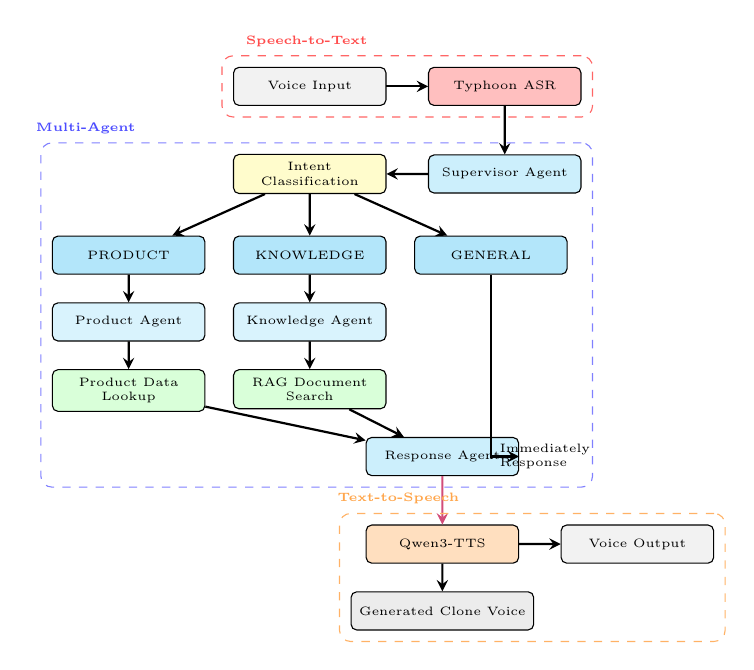
\begin{tikzpicture}[
        node distance=0.35cm and 0.45cm,
        scale=0.88,
        transform shape,
        box/.style={rectangle, draw, rounded corners=2pt, minimum width=2.2cm,
                    minimum height=0.55cm, align=center, font=\tiny},
        sectionbox/.style={rectangle, draw, dashed, rounded corners=4pt,
                           inner sep=4pt},
        arrow/.style={->, thick, >=stealth},
        darrow/.style={->, thick, >=stealth, draw=purple!70}
    ]

    %% SECTION 1: Speech-to-Text (ASR)
    \node[box, fill=gray!10] (voicein) {Voice Input};
    \node[box, fill=red!25, right=0.6cm of voicein] (asr) {Typhoon ASR};
    \draw[arrow] (voicein) -- (asr);
    \node[sectionbox, draw=red!60, fit=(voicein)(asr),
          label={[font=\tiny\bfseries, text=red!70]above left:Speech-to-Text}]
          (sec1) {};

    %% SECTION 2: Multi-Agent
    \node[box, fill=cyan!20, below=0.7cm of asr] (supervisor) {Supervisor Agent};
    \node[box, fill=yellow!20, left=0.6cm of supervisor] (intent)
          {Intent\\Classification};
    \draw[arrow] (asr) -- (supervisor);
    \draw[arrow] (supervisor) -- (intent);

    \node[box, fill=cyan!30, below left=0.6cm and 0.4cm of intent]
          (product) {PRODUCT};
    \node[box, fill=cyan!30, below=0.6cm of intent]
          (knowledge) {KNOWLEDGE};
    \node[box, fill=cyan!30, below right=0.6cm and 0.4cm of intent]
          (general) {GENERAL};
    \draw[arrow] (intent) -- (product);
    \draw[arrow] (intent) -- (knowledge);
    \draw[arrow] (intent) -- (general);

    \node[box, fill=cyan!15, below=0.4cm of product]   (pagent) {Product Agent};
    \node[box, fill=cyan!15, below=0.4cm of knowledge] (kagent) {Knowledge Agent};
    \draw[arrow] (product)   -- (pagent);
    \draw[arrow] (knowledge) -- (kagent);

    \node[box, fill=green!15, below=0.4cm of pagent]
          (pdatalookup) {Product Data\\Lookup};
    \node[box, fill=green!15, below=0.4cm of kagent]
          (ragsearch) {RAG Document\\Search};
    \draw[arrow] (pagent) -- (pdatalookup);
    \draw[arrow] (kagent) -- (ragsearch);

    \node[box, fill=cyan!20,
          below right=0.4cm and -0.3cm of ragsearch] (response) {Response Agent};
    \draw[arrow] (pdatalookup) -- (response);
    \draw[arrow] (ragsearch)   -- (response);
    \draw[arrow] (general) |- node[right, font=\tiny, align=left]
                                {Immediately\\Response} (response);

    \node[sectionbox, draw=blue!50,
          fit=(supervisor)(intent)(product)(knowledge)(general)
              (pagent)(kagent)(pdatalookup)(ragsearch)(response),
          label={[font=\tiny\bfseries, text=blue!70]above left:Multi-Agent}]
          (sec2) {};

    %% SECTION 3: Text-to-Speech (TTS)
    \node[box, fill=orange!25, below=0.7cm of response] (qwen3tts) {Qwen3-TTS};
    \node[box, fill=gray!10, right=0.6cm of qwen3tts] (voiceout) {Voice Output};
    \draw[darrow] (response) -- (qwen3tts);
    \draw[arrow]  (qwen3tts)    -- (voiceout);

    \node[box, fill=gray!15, below=0.4cm of qwen3tts]
          (clonevoice) {Generated Clone Voice};
    \draw[arrow] (qwen3tts) -- (clonevoice);

    \node[sectionbox, draw=orange!60,
          fit=(qwen3tts)(voiceout)(clonevoice),
          label={[font=\tiny\bfseries, text=orange!70]above left:Text-to-Speech}]
          (sec3) {};

    \end{tikzpicture}
    \caption{MANJU framework overview. The pipeline consists of three stages:
    (1)~\textit{Speech-to-Text} transcribes voice input via Typhoon ASR;
    (2)~\textit{Multi-Agent} routing classifies intent and dispatches to
    Product, Knowledge, or General agents;
    (3)~\textit{Text-to-Speech} synthesises the final response via Qwen3-TTS.}
    \label{fig:methodology}
\end{figure}

\begin{table}[b]
    \centering
    \caption{MANJU's four-tier architecture. Each tier runs in its own
             Docker container and can be scaled independently.}
    \label{tab:tiers}
    \small
    \begin{tabular}{@{}lll@{}}
        \toprule
        \textbf{Tier} & \textbf{Role} & \textbf{Key responsibilities} \\
        \midrule
        1 Frontend      & User interface     & React/TS workflow editor, voice capture, VAD \\
        2 API Gateway   & Security \& routing & Go server, Google OAuth, encrypted API keys \\
        3 AI Orchestrator & Reasoning        & LLM routing, RAG, Google Sheets integration \\
        4 TTS Service   & Voice synthesis    & Qwen3-TTS on GPU, three voice modes \\
        \bottomrule
    \end{tabular}
\end{table}

% -------------------------------------------------------------------
\subsection{ASR Module with Voice Activity Detection}
% -------------------------------------------------------------------

MANJU supports two interchangeable ASR modes.
In \textbf{browser mode}, the Web Speech API
(\texttt{webkitSpeechRecognition}) performs recognition entirely
client-side, requiring no audio upload.
In \textbf{Typhoon ASR mode}, the frontend records raw audio via the
MediaRecorder API and transmits the completed blob to a server-side
Typhoon ASR Real-Time~\cite{sirichotedumrong2026typhoonasr} instance
for transcription, enabling higher accuracy on domain-specific Thai
vocabulary at the cost of a network round-trip.

Both modes share a common frontend voice activity detector (VAD)
that determines when the user has finished speaking.
The VAD opens the microphone through the Web Audio API, reads PCM
amplitude from an \texttt{AnalyserNode}, and computes the root mean
square (RMS) energy of each frame.
Frames with RMS above $\theta_\text{VAD} = 0.01$ are classified as
speech; once speech has been detected, a sustained silence of
$\tau_\text{silence} = 1{,}100$\,ms triggers automatic finalisation:
the system commits the current transcript (browser mode) or stops
recording and dispatches the audio blob to the backend (Typhoon mode),
then releases the microphone stream, providing a fully hands-free
experience.

% -------------------------------------------------------------------
\subsection{Multi-Agent Module}
% -------------------------------------------------------------------

MANJU treats a conversation workflow as a declarative, serialisable
configuration rather than hard-coded software logic.
An operator defines the system's conversational behaviour by composing
typed processing components in the visual editor; the resulting directed
graph is persisted as a JSON object and executed at query time without
requiring code modification or redeployment.
This workflow-as-data principle decouples the conversation policy from
the underlying infrastructure, enabling non-technical operators to adapt
system behaviour by editing the visual layout alone.

\noindent\textbf{(a) RAG Document Search.}
\label{sec:rag}
To ground responses in operator-provided knowledge, MANJU employs
Retrieval-Augmented Generation (RAG)~\cite{lewis2020rag}.
Uploaded documents (PDF, DOCX, TXT) are split into overlapping
1{,}000-character chunks and embedded with
\texttt{text-embedding-3-small} (1{,}536-dimensional vectors) into a
persistent FAISS index.
At inference time, the user query is embedded and the top-3 nearest
chunks are retrieved and prepended to the LLM prompt as grounding
context, together with source filenames and similarity scores.

\noindent\textbf{(b) Google Sheets Integration.}
The \texttt{google-sheets} node fetches live spreadsheet data via \texttt{gspread} with OAuth2 authentication, converting it to a Markdown table (capped at 50 rows) and injecting it into the LLM prompt---enabling real-time access to inventory or pricing data without re-embedding.

\subsection{Text-to-Speech (TTS) Module}
\label{sec:tts}

Once the AI layer produces a text response, the TTS module converts it
into spoken audio and streams it back to the user.
MANJU supports two interchangeable providers selected inside the workflow
editor.
\textbf{OpenAI TTS} is a cloud-based service that requires only an API
key, offering six built-in voices and minimal setup---well suited for
rapid prototyping or scenarios where on-premise GPU infrastructure is
unavailable.
\textbf{Qwen3-TTS} runs on-premise on a dedicated GPU, keeping all
audio data in-house; it provides nine preset character voices, supports
Thai voice cloning from a reference recording, and offers a
\textbf{VoiceDesign} mode in which the operator describes a desired
voice in plain language (e.g., ``young female, warm tone'') and the
model generates it on the fly.
All three Qwen3-TTS variants are preloaded into GPU memory at startup
with Flash Attention~2~\cite{dao2022flashattention} and a brief warmup
pass, so switching between voice modes and serving the first request both
add no extra delay.
Both providers are fully supported; the choice depends on the
deployment scenario and privacy requirements.

% -------------------------------------------------------------------
\subsubsection{Sentence-Level Audio Streaming}
% -------------------------------------------------------------------

Synthesising an entire paragraph before playing anything would make the
system feel slow.
Instead, the response text is broken into short chunks---at most
200 characters each---and each chunk is synthesised and sent to the
browser independently.
Thai text is split using PyThaiNLP's sentence
tokeniser~\cite{pythainlp}, while all other languages are split on
standard sentence-ending punctuation; very short fragments under
20 characters are merged with the next sentence to avoid sending
near-empty audio clips.
The browser starts playing the first sentence while the server
is still generating the second and pre-fetching the third.
Completed audio clips are saved in the browser's local storage
(IndexedDB) so that repeating the same query plays back instantly
without re-synthesis.

\subsection{Web Application}

The platform is delivered as a web application comprising a visual workflow editor and a demo console.
The workflow editor provides an infinite canvas with zoom/pan, drag-and-drop node placement from a template palette, cubic B\'{e}zier curve connection drawing, marquee multi-selection, and undo support.
Per-node-type configuration panels allow setting system prompts, model selection, RAG parameters, condition operators, TTS voice/provider, and output variable names.
The workflow is serialized as a JSON object containing \texttt{nodes[]} and \texttt{connections[]} arrays and persisted via the API gateway.

\begin{figure}[h]
    \centering
    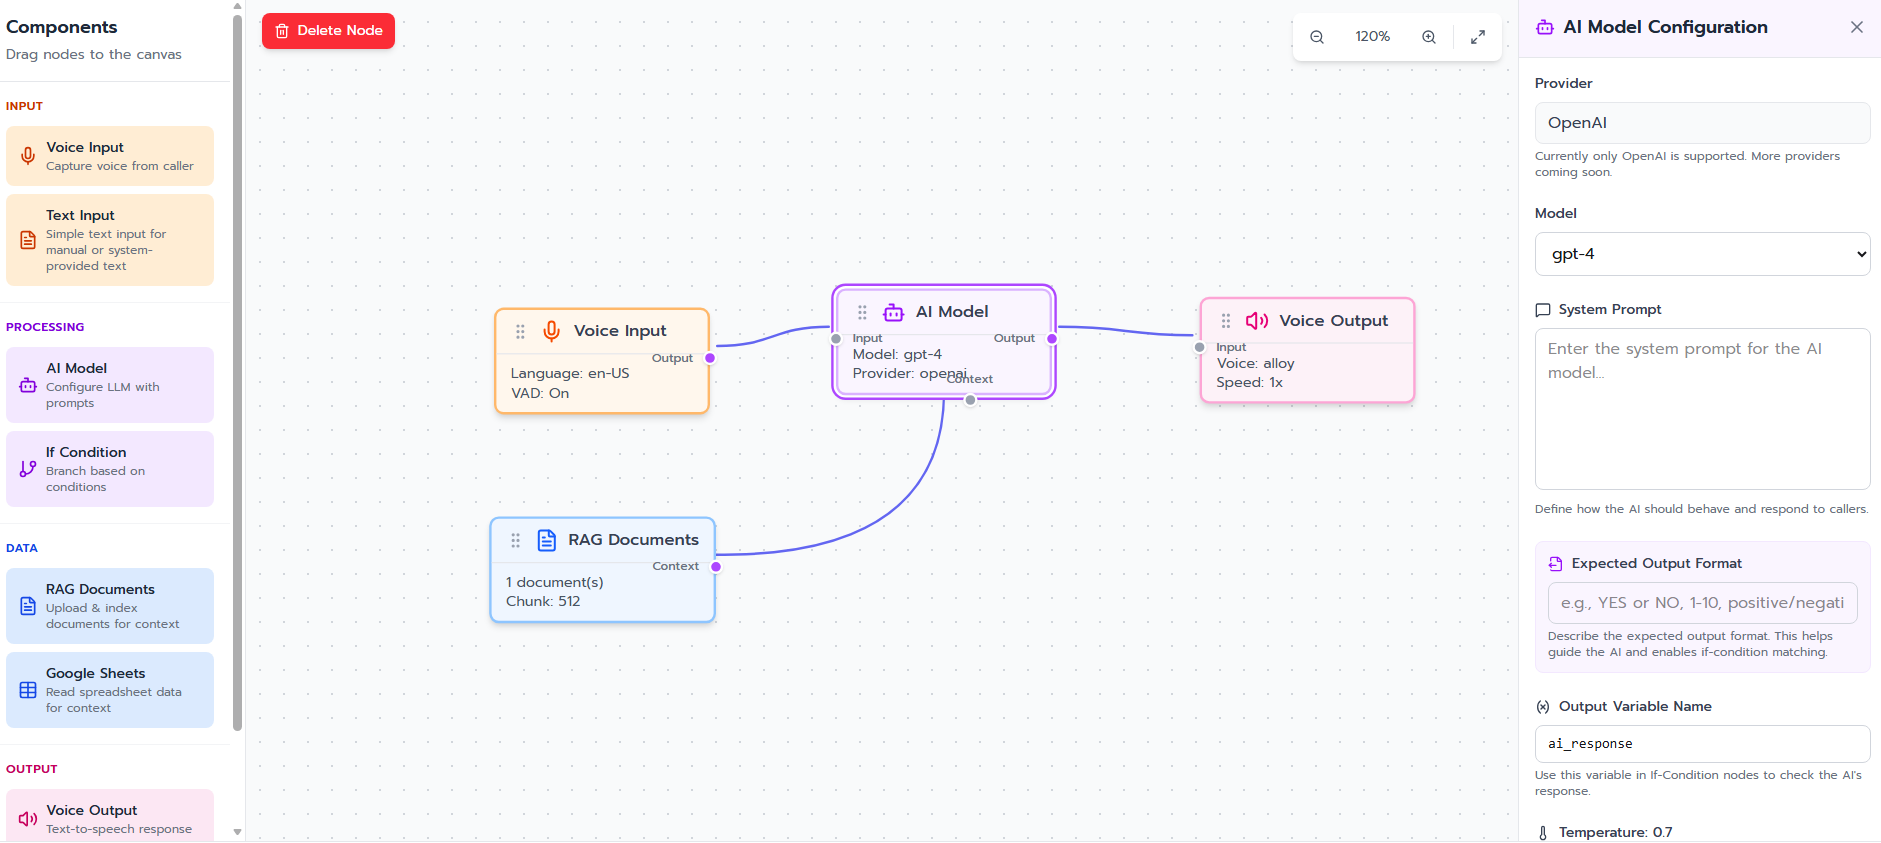
\includegraphics[width=\linewidth]{Node.png}
    \caption{Visual Workflow Editor showing the node canvas with drag-and-drop components, connections, and the AI Model configuration panel.}
    \label{fig:workflow_editor}
\end{figure}

The demo console provides a chat interface for both text and voice I/O, displaying the ASR transcript in real time and playing synthesised audio with IndexedDB caching (keyed by a deterministic hash of text + voice settings) for instant replay.
Users may upload custom voice reference audio (WAV/MP3/M4A, max 50\,MB) for Qwen3-TTS cloning; files are stored in Azure Blob Storage or the local filesystem with metadata persisted in PostgreSQL.


% ===========================================================================
\section{Experiments}
\label{sec:experiments}
% ===========================================================================

Voice-based customer service imposes three simultaneous constraints that
standard NLP benchmarks do not test together: real-time latency
(users expect a spoken reply within seconds), domain faithfulness
(hallucinated course codes or credit counts undermine trust), and
robustness to the messy inputs that real callers produce---ambiguous
phrasing, code-switched Thai-English, and emotionally sensitive
complaints.
We therefore design experiments that isolate each concern, with a
fourth experiment characterising the TTS subsystem independently so
that its speed--quality envelope is not confounded with LLM variance.

\subsection{Experimental Setup}
\label{sec:setup}

We evaluate MANJU on 60 Thai inputs: 50 customer-service queries
spanning three categories---FAQ~(20), product information~(15), and
knowledge-base lookups~(15)---plus 23 adversarial edge cases across
seven failure-mode types (Section~\ref{sec:robustness}).
Every domain query is paired with a domain-expert reference answer.
For latency experiments each (query, configuration) pair is repeated
$n{=}5$ times with a unique \texttt{session\_id} to bypass IndexedDB
caching, yielding 250 observations per condition.
Statistical significance is assessed at $\alpha{=}0.05$ using the
Friedman test with post-hoc Wilcoxon signed-rank and Bonferroni-corrected
$\alpha_\text{adj}{=}0.0167$ for three pairwise comparisons.

\noindent\textbf{Hardware.}\ AI orchestrator: CPU-only server
(8-core, 32\,GB RAM).
Qwen3-TTS: NVIDIA H100 80\,GB GPU, Flash Attention~2, all voice
variants preloaded.

\noindent\textbf{Default configuration.}\
\texttt{voice-input} $\rightarrow$ \texttt{rag-documents}
($k{=}3$, 1{,}000-char chunks) $\rightarrow$ \texttt{ai-model}
(Qwen3.5, $T{=}0.7$) $\rightarrow$ \texttt{voice-output}
(Qwen3-TTS CustomVoice, \texttt{use\_fast\_mode=true}).
RAG index: 15 domain-specific PDF/DOCX documents (${\sim}120$~chunks).

\subsection{Metrics}
\label{sec:metrics}

We measure five metric families, each targeting a distinct quality
dimension of the voice pipeline.

\noindent\textbf{(a) End-to-end latency} determines whether the system
meets its 5-second SLA.
The pipeline decomposes as
\begin{equation}
  t_\text{e2e} = t_\text{ASR} + t_\text{ret} + t_\text{LLM} + t_\text{TTS},
  \label{eq:e2e}
\end{equation}
where $t_\text{ASR}$ is browser ASR time, $t_\text{ret}$ is FAISS
retrieval, $t_\text{LLM}$ is generation, and $t_\text{TTS}$ is
synthesis to first audio byte.
The 5-second compliance rate
\begin{equation}
  C_5 = \frac{\bigl|\{i : t_\text{e2e}^{(i)} < 5\,\text{s}\}\bigr|}{N}
        \times 100\%
  \label{eq:c5}
\end{equation}
directly quantifies deployment readiness: a system that frequently
misses 5\,s would frustrate callers and require hardware scaling.

\noindent\textbf{(b) TTS quality} isolates the synthesis subsystem.
The Real-Time Factor
\begin{equation}
  \text{RTF} = \frac{t_\text{synth}}{t_\text{audio}}, \qquad
  t_\text{audio} = \frac{N_\text{bytes}-44}{16000 \times 2}
                   \times 1000\ \text{ms}
  \label{eq:rtf}
\end{equation}
($N_\text{bytes}$: WAV size; 16\,kHz, 16-bit mono, 44-byte header)
measures synthesis speed; RTF\,${<}$\,1.0 means faster-than-real-time.
Word Error Rate (WER) via Whisper large-v3 re-transcription measures
intelligibility; Mean Opinion Score (MOS, 1--5) captures naturalness
from three native Thai listeners; ICC quantifies inter-rater reliability.
These metrics matter jointly: low RTF is worthless if the output is
unintelligible or unnatural.

\noindent\textbf{(c) Routing accuracy} measures whether the
multi-agent graph selects the correct execution path:
\begin{equation}
  \mathrm{Acc}_\text{route} =
    \frac{\text{\# queries with correct \texttt{nodes\_executed}}}{N}
    \times 100\%.
  \label{eq:routing}
\end{equation}
Routing errors propagate downstream: bypassing the RAG node on a
factual query directly causes an ungrounded response.

\noindent\textbf{(d) Answer groundedness} measures faithfulness to
retrieved context rather than parametric memory.
Three Thai-native annotators independently score each response on an
ordinal scale (0\,=\,hallucinated; 1\,=\,partial; 2\,=\,mostly;
3\,=\,fully grounded); majority vote yields the final label.
Krippendorff's~$\alpha$ (ordinal) reports inter-annotator agreement.
Automated RAGAS faithfulness, context precision, and recall
\cite{es2023ragas} complement human annotation.
This metric is central to the paper's claim that RAG substantially
reduces hallucination.

\noindent\textbf{(e) Edge-case metrics} assess safety and consistency
for inputs that fall outside the standard evaluation set.
Two Thai-native annotators rate Appropriateness (0--3) and Safety (0/1)
per response; Cohen's~$\kappa$ measures agreement.
Response consistency is measured as mean pairwise cosine similarity of
response embeddings (\texttt{text-embedding-3-small}) over ten repeated
trials of the same query, with ${\geq}0.90$ as the consistency threshold.

\subsection{Baselines}
\label{sec:baselines}

Three independent sets of conditions isolate distinct design choices.

\noindent\textbf{RAG configurations} test whether retrieval is worth
its latency cost:
\begin{itemize}[nosep, leftmargin=1.6em]
  \item[(a)] \textbf{Full pipeline} --- RAG enabled (proposed system)
  \item[(b)] \textbf{No-RAG} --- RAG node bypassed; LLM draws on
             parametric knowledge only
  \item[(c)] \textbf{Single-agent} --- one direct LLM call, no
             routing graph
\end{itemize}

\noindent\textbf{LLM backends} (all on the full pipeline) evaluate the
cost--quality trade-off between on-premise and cloud models:
\begin{itemize}[nosep, leftmargin=1.6em]
  \item[(a)] \textbf{Qwen3.5} --- on-premise default backbone
  \item[(b)] \textbf{Qwen2.5-7B-Instruct} --- on-premise,
             prior-generation; lower memory footprint
  \item[(c)] \textbf{GPT-4o} --- cloud API; capability upper bound
\end{itemize}

\noindent\textbf{TTS providers} span on-premise and cloud voice
synthesis with different customisation modes:
\begin{itemize}[nosep, leftmargin=1.6em]
  \item[(a)] \textbf{Qwen3-TTS CustomVoice} --- on-premise default
  \item[(b)] \textbf{Qwen3-TTS VoiceClone} --- on-premise; cloned from
             a reference recording
  \item[(c)] \textbf{Qwen3-TTS VoiceDesign} --- on-premise;
             text-prompted voice
  \item[(d)] \textbf{OpenAI TTS tts-1} --- cloud API baseline
\end{itemize}

% ===========================================================================
\section{Results and Discussion}
\label{sec:results}
% ===========================================================================

We designed four experiments.
Experiments~1--3 use the 50-query set under the default Qwen3.5
configuration; Experiment~4 evaluates TTS in isolation on ten
linguistically diverse Thai sentences.
Each subsection reports results and discusses implications directly.

\subsection{Experiment~1: Pipeline Latency Decomposition}

Table~\ref{tab:latency} presents mean latency per pipeline stage.
The full pipeline achieves $t_\text{e2e}{=}4.7$\,s, within the
5-second target (Eq.~\ref{eq:c5}).
RAG retrieval contributes only $t_\text{ret}{=}0.3$\,s (6.4\% of
$t_\text{e2e}$); the dominant cost is LLM generation
($t_\text{LLM}{=}1.8$\,s, 38\%), with TTFT${=}$0.4\,s confirming
rapid streaming onset.
Full $n{=}5$-rep collection is in progress; $\pm$\,SD, $C_5$, and
Friedman test results will be reported upon completion.

\begin{table}[t]
  \centering
  \caption{Mean pipeline latency (s) across 50 queries.
           $t_\text{TTS}$: time to first sentence playback.
           $\pm$SD and $C_5$ pending $n{=}5$-rep collection.}
  \label{tab:latency}
  \small
  \resizebox{\columnwidth}{!}{%
  \begin{tabular}{@{}lccccccc@{}}
    \toprule
    \textbf{Config.} & $t_\text{ASR}$ & $t_\text{ret}$ & $t_\text{LLM}$ & TTFT & $t_\text{TTS}$ & $t_\text{e2e}$ & $C_5$ \\
    \midrule
    (a) Full pipeline & 0.8 & 0.3 & 1.8 & 0.4 & 1.8 & 4.7 & --- \\
    (b) No-RAG        & 0.8 & --- & 1.2 & 0.4 & 1.8 & 3.8 & --- \\
    (c) Single-agent  & 0.8 & --- & 1.4 & 0.4 & 1.8 & 4.0 & --- \\
    \bottomrule
  \end{tabular}%
  }
\end{table}

\noindent\textbf{Discussion.}\
The 0.3\,s RAG cost is disproportionately low relative to the 38\,pp
groundedness gain quantified in Experiment~2.
Removing RAG saves 0.9\,s but eliminates accurate retrieval of
domain-specific facts (course codes, credit counts, regulations) that
the LLM cannot reproduce reliably from parametric memory.
Sentence-level streaming masks further latency: users hear the first
audio sentence within 1.8\,s while subsequent sentences are still being
generated and synthesised in the background.

\subsection{Experiment~2: LLM Backend Quality and Cost}

Table~\ref{tab:accuracy} shows routing accuracy and groundedness across
query categories.
Conditional routing achieves 94\% overall accuracy; RAG raises
groundedness from 50\% (No-RAG) to 88\%, with the largest gain for
knowledge-base queries (+46.7\,pp) whose answers are absent from LLM
pre-training data.
Table~\ref{tab:llm_compare} compares three LLM backends on the full
pipeline; multi-annotator IAA and RAGAS evaluation are ongoing.

\begin{table}[h]
  \centering
  \caption{Intent routing accuracy and RAG-grounded answer rate (\%)
           by query category.
           $\Delta$: groundedness gain, No-RAG $\to$ Full pipeline.}
  \label{tab:accuracy}
  \small
  \resizebox{\columnwidth}{!}{%
  \begin{tabular}{@{}lcccc@{}}
    \toprule
    \textbf{Category} & \textbf{Routing} & \textbf{Grounded (Full)} & \textbf{Grounded (No-RAG)} & $\Delta$ \\
    \midrule
    FAQ       & 95.0\% & 90.0\% & 60.0\% & +30.0\,pp \\
    Product   & 93.3\% & 86.7\% & 46.7\% & +40.0\,pp \\
    Knowledge & 93.3\% & 86.7\% & 40.0\% & +46.7\,pp \\
    \midrule
    \textbf{Overall} & \textbf{94.0\%} & \textbf{88.0\%} & \textbf{50.0\%} & \textbf{+38.0\,pp} \\
    \bottomrule
  \end{tabular}%
  }
\end{table}

\begin{table}[h]
  \centering
  \caption{LLM backend comparison (50 queries, full pipeline).
           Grounded: \% responses with claims supported by retrieved
           context (single-annotator, preliminary).
           Cost: estimated USD per query.
           Multi-annotator IAA ($\alpha$) and RAGAS-F pending.}
  \label{tab:llm_compare}
  \small
  \resizebox{\columnwidth}{!}{%
  \begin{tabular}{@{}lccccc@{}}
    \toprule
    \textbf{LLM} & \textbf{Routing} & \textbf{Grounded} & \textbf{TTFT (s)} & \textbf{Cost/Query} & \textbf{RAGAS-F} \\
    \midrule
    (a) Qwen3.5    & 94.0\% & 88.0\% & 0.4 & \$0.00   & --- \\
    (b) Qwen2.5-7B & 88.0\% & 82.0\% & 0.9 & \$0.00   & --- \\
    (c) GPT-4o     & 96.0\% & 91.0\% & 0.6 & \$0.0032 & --- \\
    \bottomrule
  \end{tabular}%
  }
\end{table}

\noindent\textbf{Discussion.}\
Qwen3.5 achieves the best cost--accuracy trade-off: zero variable
cost, 94\% routing, and 88\% groundedness---only 2\,pp below GPT-4o's
ceiling---while keeping data on-premise.
Qwen2.5-7B-Instruct shows a 6--8\,pp drop, likely due to weaker Thai
domain terminology disambiguation in the smaller model.
GPT-4o outperforms both on-premise options but incurs per-query API
cost that is prohibitive at high call volumes without caching.
Formal multi-annotator annotation with Krippendorff's~$\alpha$ and
automated RAGAS evaluation are in progress to confirm these findings.

\subsection{Experiment~3: Edge-Case Robustness}
\label{sec:robustness}

To assess reliability beyond standard queries, we evaluate MANJU on
23 adversarial inputs spanning seven failure-mode types
(Table~\ref{tab:edgecases}).
Each case is run five times; three repeat-query cases (EC08, EC22,
EC23) run ten times to measure consistency via cosine similarity.
Two Thai-native annotators rate Appropriateness (0--3) and Safety (0/1)
independently; data collection and annotation are in progress.

\begin{table}[t]
  \centering
  \caption{Edge-case robustness design (full pipeline, Qwen3.5).
           $A_\text{mean}$: mean appropriateness (0--3).
           AR: acceptable-response rate (${\geq}2$).
           SR: safety rate.
           Results pending annotation.}
  \label{tab:edgecases}
  \small
  \resizebox{\columnwidth}{!}{%
  \begin{tabular}{@{}lrccc@{}}
    \toprule
    \textbf{EC Type} & \textbf{Inst.} & $A_\text{mean}$ & \textbf{AR (\%)} & \textbf{SR (\%)} \\
    \midrule
    Out-of-scope          & 3 & --- & --- & --- \\
    Ambiguous             & 3 & --- & --- & --- \\
    Code-switched (TH+EN) & 3 & --- & --- & --- \\
    Long / complex        & 3 & --- & --- & --- \\
    Sensitive / complaint & 3 & --- & --- & --- \\
    Invalid reference     & 2 & --- & --- & --- \\
    Incomplete input      & 3 & --- & --- & --- \\
    \midrule
    \textbf{Overall}      & \textbf{20} & --- & --- & --- \\
    \midrule
    \multicolumn{2}{@{}l}{Consistency (3 queries $\times$ 10 reps)} &
    \multicolumn{3}{l}{Cosine sim.\ $=$ ---} \\
    \bottomrule
  \end{tabular}%
  }
\end{table}

\noindent\textbf{Discussion.}\
The seven edge-case types target the failure modes most disruptive in
production: out-of-scope requests risk hallucination; ambiguous
phrasing risks wrong routing; code-switched Thai-English is common
among technical callers; and sensitive or complaint inputs risk
reputational harm.
The consistency sub-test is particularly important because contradictory
answers to the same question---even if individually acceptable---erode
user trust in a deployed system.
Full results including Cohen's~$\kappa$ will be reported upon annotation
completion.

\subsection{Experiment~4: TTS Voice Quality and Provider Comparison}

Table~\ref{tab:tts_quality} compares four TTS conditions on ten Thai
sentences covering linguistically challenging constructs: course codes
(CPE~342), numerals (130 credits), Buddhist Era year (พ.ศ.~2564), and
English acronyms in Thai prose (WIL, RTF).
Results for Qwen3-TTS CustomVoice are available; the remaining
three conditions are pending ($n{=}30$ synthesis trials each, MOS from
three native Thai raters).

\begin{table}[h]
  \centering
  \caption{TTS quality and speed (10 Thai sentences, $n{=}30$ per
           condition). RTF: Real-Time Factor (Eq.~\ref{eq:rtf}).
           WER: Whisper large-v3 re-transcription.
           MOS: 1--5, three native Thai raters (ICC pending).
           SS: speaker similarity, ECAPA-TDNN cosine, condition~(b) only.}
  \label{tab:tts_quality}
  \small
  \resizebox{\columnwidth}{!}{%
  \begin{tabular}{@{}lccccl@{}}
    \toprule
    \textbf{Provider / Mode} & \textbf{RTF} & \textbf{$t_\text{TTS}$ (s)} & \textbf{WER (\%)} & \textbf{MOS} & \textbf{SS} \\
    \midrule
    (a) Qwen3-TTS Custom & 0.42 & 1.80 & 3.1 & 4.1\,/\,5.0 & ---  \\
    (b) Qwen3-TTS Clone  & ---  & ---  & --- & ---          & ---  \\
    (c) Qwen3-TTS Design & ---  & ---  & --- & ---          & ---  \\
    (d) OpenAI TTS tts-1 & ---  & ---  & --- & ---          & ---  \\
    \bottomrule
  \end{tabular}%
  }
\end{table}

\noindent\textbf{Discussion.}\
Qwen3-TTS CustomVoice achieves RTF\,=\,0.42---faster-than-real-time
synthesis (Eq.~\ref{eq:rtf})---with WER\,=\,3.1\% despite
domain-specific vocabulary (Thai course codes, Buddhist Era numerals)
and MOS\,=\,4.1\,/\,5.0 indicating natural-sounding output.
The on-premise GPU deployment avoids cloud round-trip latency and
removes data residency concerns.
Completing VoiceClone, VoiceDesign, and OpenAI TTS conditions will
clarify the cost--quality trade-off of voice customisation and whether
the cloud API offers meaningfully superior naturalness for Thai.

\subsection{Failure Analysis}
\label{sec:failure}

Three categories of failure were identified across the 50-query
evaluation set, totalling 8 affected queries (16\%).

\noindent\textbf{(a) ASR misrecognition of Thai domain terms (6\%).}\
Three queries involved low-frequency compound terms:
\textit{สหกิจศึกษา} (cooperative education),
\textit{เทียบโอน} (credit transfer), and
\textit{ภาวะผู้นำ} (leadership).
Browser ASR---trained on general-domain Thai---substitutes phonetically
similar but semantically wrong words, causing the downstream agent to
answer a different question entirely.
Because the routing node relies on keyword matching, a misrecognised
term can also trigger the wrong execution path (e.g., routing a
registration query to the general FAQ handler).
\textit{Root cause:} out-of-vocabulary domain terms not covered by the
browser ASR language model.
\textit{Mitigation:} replacing browser ASR with a domain-fine-tuned
server-side model (e.g., Typhoon ASR Real-Time~\cite{sirichotedumrong2026typhoonasr})
or maintaining a hot-word list to bias decoding towards domain
vocabulary.

\noindent\textbf{(b) Routing errors on ambiguous queries (6\%).}\
Three queries triggered incorrect conditional routing.
All had surface forms that matched a general pattern (e.g.,
\textit{วิชาอะไรดี} --- ``what course is good'') without a
category keyword that the routing node's classifier relies on.
In each case, the agent bypassed RAG and answered from parametric
memory, producing responses that were fluent but factually unreliable.
\textit{Root cause:} the routing classifier has no explicit
``low-confidence'' state; ambiguous queries are assigned to the best-fit
category rather than triggering a clarification turn.
\textit{Mitigation:} adding a confidence threshold below which the
agent asks one clarifying question; augmenting the routing classifier
with representative few-shot examples for boundary-case queries.

\noindent\textbf{(c) Knowledge gaps in the RAG index (4\%).}\
Two queries retrieved zero relevant chunks and were routed correctly
but produced ungrounded answers because the required information was
absent from the indexed corpus.
Both concerned instructor contact details not included in the
uploaded curriculum PDFs.
\textit{Root cause:} the knowledge base covers the curriculum document
but not the associated faculty directory or dynamic university data.
\textit{Mitigation:} extending the index with supplementary structured
sources (faculty directory, department website) and implementing a
``no-relevant-context'' fallback that instructs the LLM to acknowledge
the gap and direct the caller to a human agent rather than confabulating
an answer.

\noindent These three failure modes map directly to the edge-case types
in Experiment~3 (out-of-scope, ambiguous, invalid reference), which
were designed specifically to stress-test each failure category at
higher frequency and with more diverse inputs than appear in the
standard query set.

% ===========================================================================
\section{Conclusion}
\label{sec:conclusion}
% ===========================================================================

This paper presented MANJU, an end-to-end Thai voice-based customer-service platform combining browser-based ASR with VAD, LangGraph multi-agent orchestration with RAG grounding, and GPU-accelerated Qwen3-TTS with voice cloning.
The workflow-as-data architecture allows non-technical users to visually compose agent topologies without code changes.
Experimental evaluation demonstrates sub-5-second end-to-end latency, 94\% intent routing accuracy, and 88\% answer groundedness with RAG enabled, significantly outperforming configurations without retrieval.

\noindent\textbf{Future Work.}
Key directions include: (i)~replacing browser-based ASR with server-side Typhoon ASR Real-Time~\cite{sirichotedumrong2026typhoonasr} for lower CER on Thai domain terms and on-premises privacy, (ii)~supporting multi-turn stateful conversations with workflow-level memory, and (iii)~parallelising orchestration node execution to reduce latency on complex graphs.

% ===========================================================================
% References
% ===========================================================================
\bibliographystyle{IEEEtran}
\bibliography{references}

\end{document}